\documentclass[a4paper,9pt]{ltjsarticle}
\usepackage{graphicx}
\usepackage{luatexja-fontspec}
\usepackage{caption}
\usepackage{amsmath,amssymb,bm,braket}
\usepackage[english]{babel}
\usepackage{multicol}
\usepackage{titlesec}
%\usepackage{gnuplot-lua-tikz}
\usepackage[top=20truemm,bottom=20truemm,left=20truemm,right=20truemm]{geometry}
\usepackage{array}
\usepackage{upgreek}
\usepackage{fancyhdr}
\renewcommand{\refname}{}
\usepackage{listings,jvlisting}
\usepackage{tikz}
\usepackage[thmmarks,amsmath]{ntheorem}
\usepackage[version=3]{mhchem}
\usetikzlibrary{external}
\tikzexternalize
\lstset{
  basicstyle={\ttfamily},
  identifierstyle={\small},
  commentstyle={\smallitshape},
  keywordstyle={\small\bfseries},
  ndkeywordstyle={\small},
  stringstyle={\small\ttfamily},
  frame={tb},
  breaklines=true,
  columns=[l]{fullflexible},
  numbers=left,
  xrightmargin=0pt,
  xleftmargin=3pt,
  numberstyle={\scriptsize},
  stepnumber=1,
  numbersep=1pt,
  lineskip=-0.5ex
}
\captionsetup[figure]{format=plain, labelformat=simple, labelsep=quad,labelfont=bf,name={Fig.}}
\captionsetup[table]{format=plain, labelformat=simple, labelsep=quad,labelfont=bf}
\parindent = 0pt
%[BoldFont=HGSMinchoE]{MSMincho}[BoldFont=HiraMinProN-W6]{HiraMinPro-W3}
\titleformat{\section}{\normalfont\fontsize{9}{10}\bfseries\fontspec{Times New Roman}}{\thesection.}{1em}{}
\usepackage[backend=biber,sorting=none,style=numeric,maxnames=99,minnames=1]{biblatex}
\addbibresource{utility/REFERENCES.bib}
\defbibheading{bibliography}[\refname]{%
  \section*{REFERENCES}%
  \vspace{-7pt}  % ここで空白を調整。お好みの値に変更してください。
}
\newfontfamily\subsectionfont{Times New Roman} % サブセクション用フォント
\titleformat{\subsection}
  {\normalfont\large\bfseries} % サブセクションのフォントを指定
  {\thesubsection}{1em}{}
\renewbibmacro{in:}{}
\renewbibmacro*{journal+issuetitle}{%
  \addcomma\space% カンマとスペースを追加
  \usebibmacro{journal}%
  \setunit*{\addspace}%
  \usebibmacro{volume+number+eid}%
  \setunit{\addspace}%
  \printfield{note}%
  \newunit
}
\renewbibmacro*{volume+number+eid}{
  \printfield{volume}%
  \setunit*{\addnbspace}%
  \printfield{number}%
  \setunit{\addcomma\space}%
  \printfield{eid}
}
\DeclareFieldFormat[article]{volume}{\textbf{#1}}
\DeclareFieldFormat[article]{pages}{#1}
\DeclareFieldFormat{journaltitle}{#1}
\usepackage{hyperref}
\renewenvironment{abstract}{\par\noindent}{\par}
%\pagenumbering{gobble}
\usepackage{docmute}
\usepackage{setspace}
\usepackage{titlesec} % 見出しのカスタマイズ用

% セクションのフォーマットをカスタマイズ
\titleformat{\section}
  {} % フォントサイズとスタイル
  {\Large\bfseries\thesection\ \ }               % 番号の前の内容(空白)
  {0em}            % 番号とタイトルの間の間隔
  {\Large\bfseries}


\theoremstyle{plain}
\theoremheaderfont{\normalfont\bfseries}
\theorembodyfont{\itshape}   % 本文を斜体に
\theoremseparator{.}         % タイトルと本文の区切りを「.」に設定
\newtheorem{definition}{Definition}
\begin{document}
\centerline{\Large\bfseries Dynamical Codeによるunfolding Color Code}
\vspace{10pt}
 FuとGottesmanのError Correction in Dynamical Codes(Dynamical CodeはおそらくSubsystemとFloquet Codeの総称) \cite{fu2024}の前半部分を参考にして、GidneyのMagic State Cultivation \cite{gidney2024}のColor CodeからSurface Codeへのescapeを考えてみた。


\section{Dynamical CodeによるColor Codeのunfolding (Color Code → Surface Code)}{
     ここでは、Fig.\ref{figure1}のような符号距離5のColor Codeについて考える。\\

    \begin{figure}[h]
        \centering
        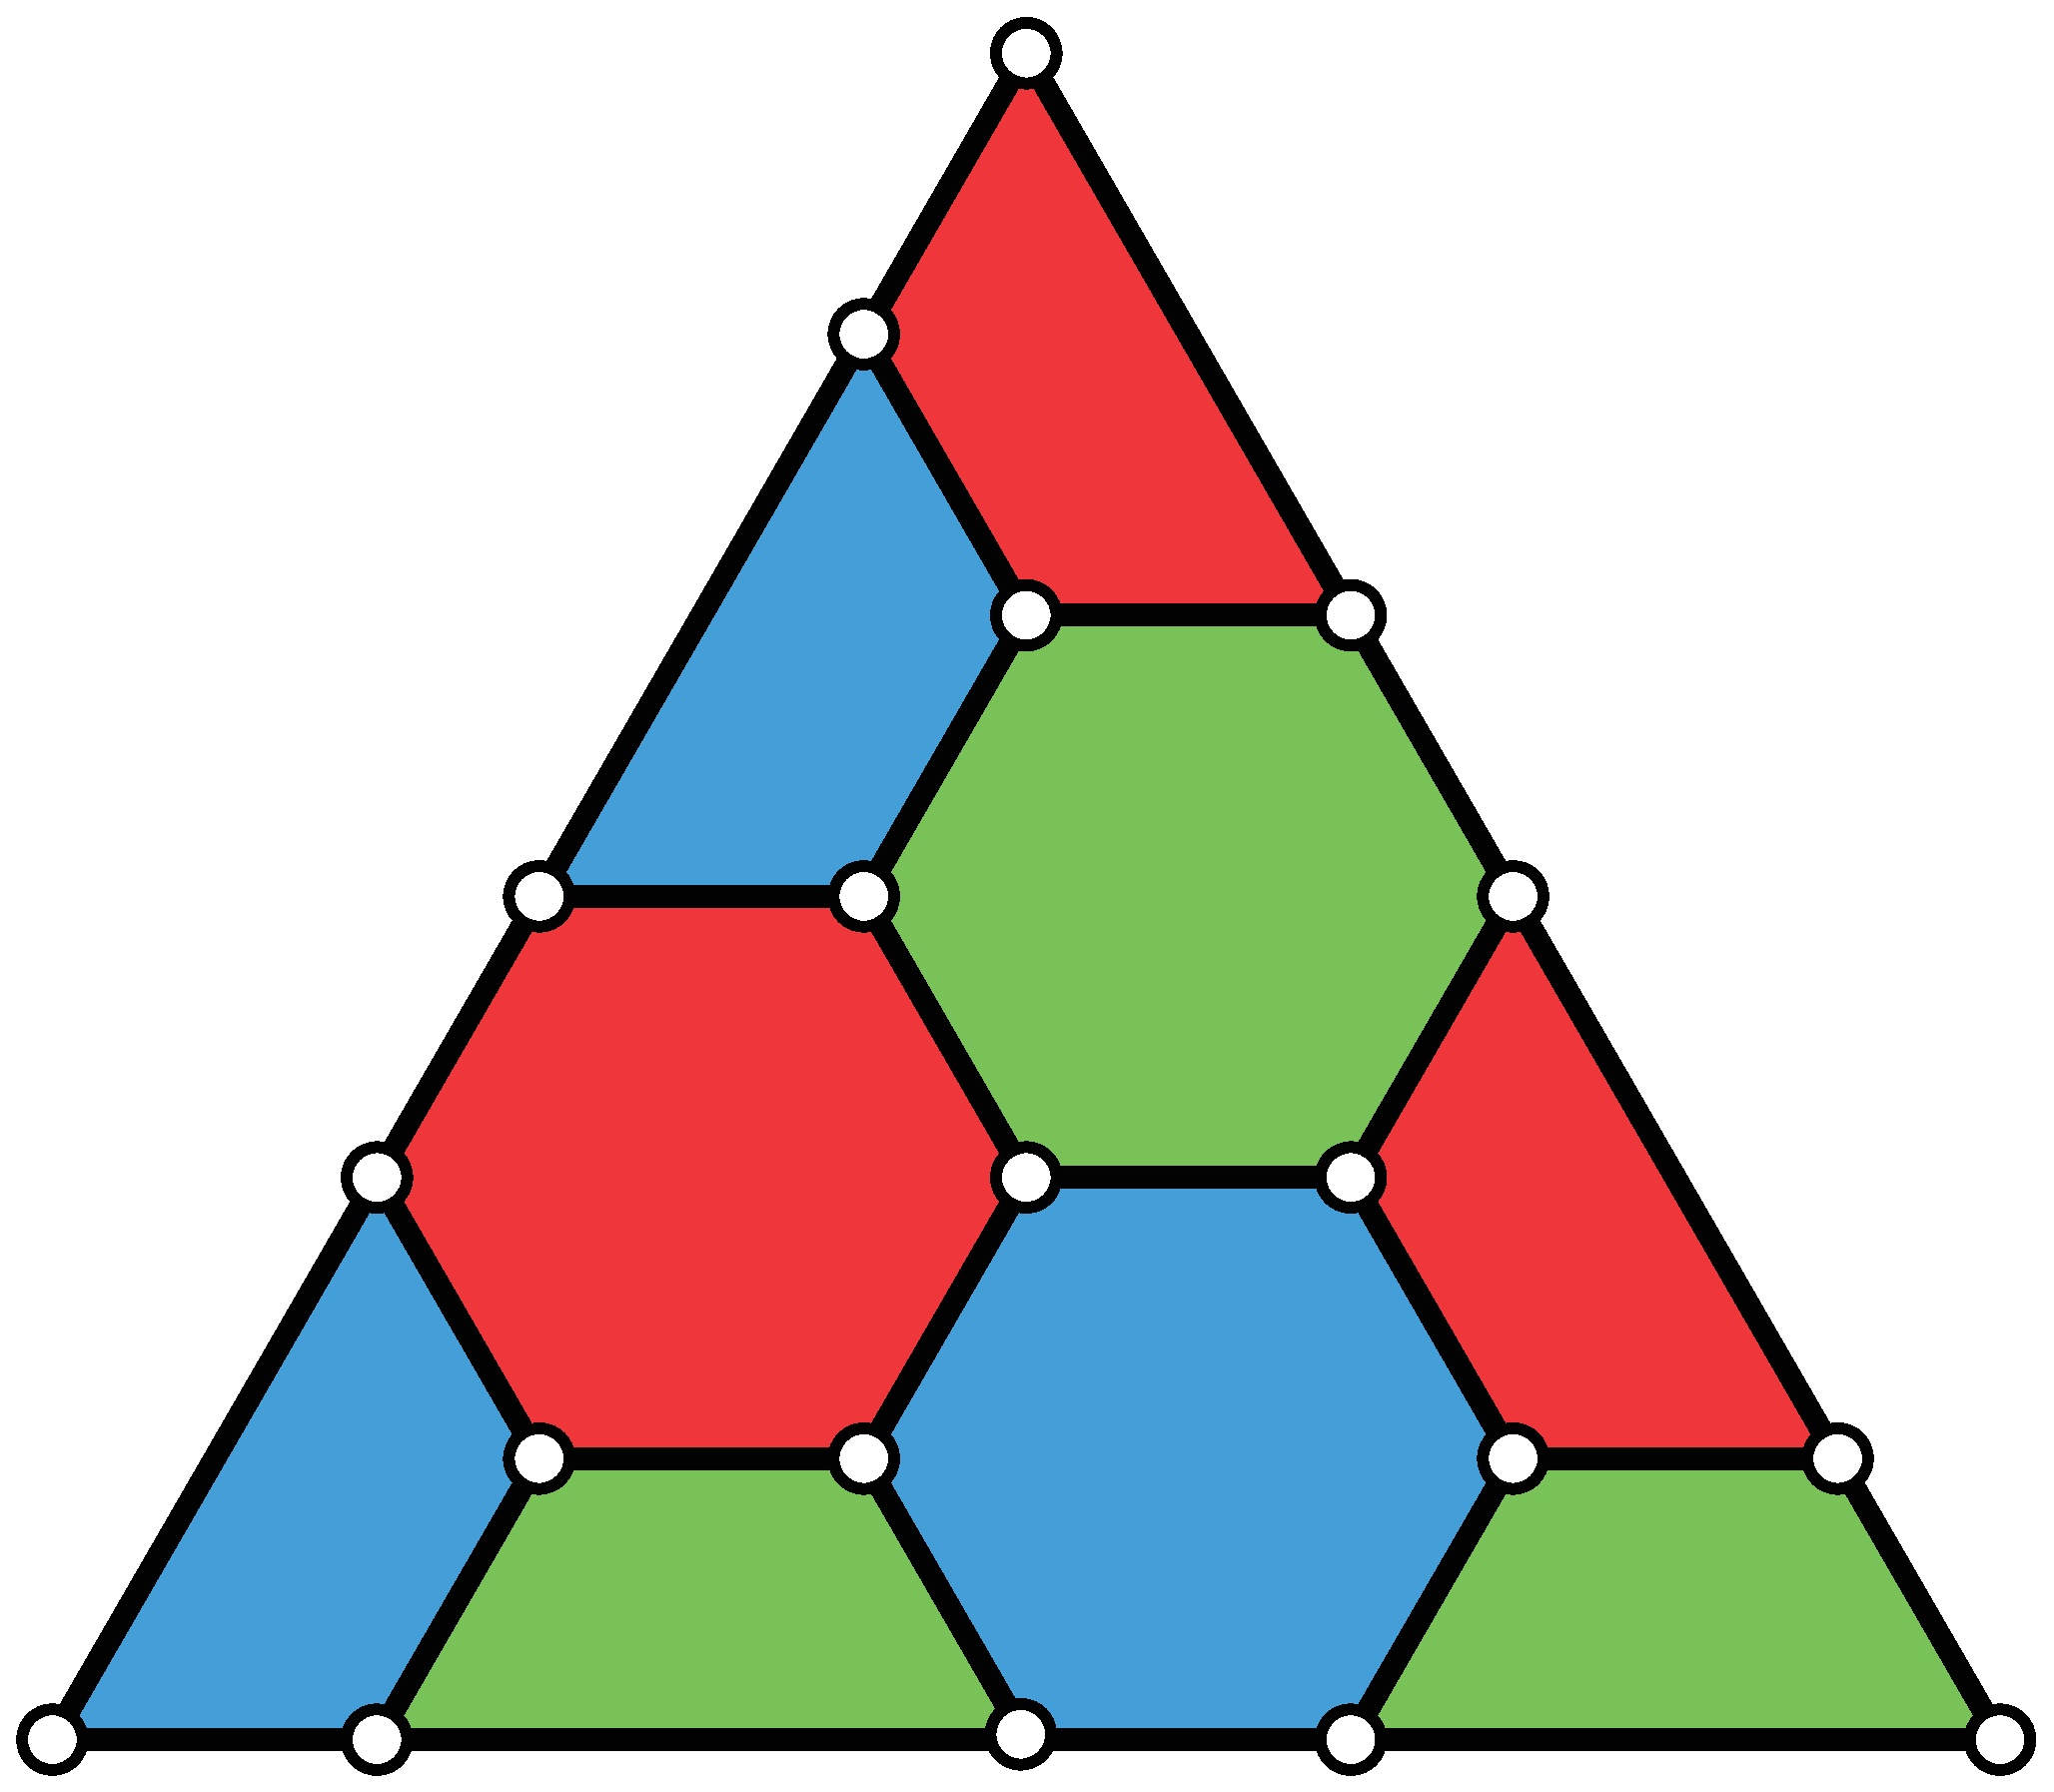
\includegraphics[scale=0.15]{figure/figure1.eps}
        \vspace{10pt}\caption{}
        \label{figure1}
        \vspace{-15pt}
    \end{figure}

    最初にColor CodeのX logical operatorをgreen boundaryに沿う5-weight operator、Z logaical operatorをred boundaryに沿う5-weight operatorと定義する。
    ここではColor CodeをFig.\ref{figure1}のblue boundaryを折り目として開くことを考える。Color Codeをunfoldする直前はFig.\ref{figure2}のように折り目のboudary側に0初期化された量子ビットを、unfoldするColor Codeの量子ビット数nから符号距離dを引いた$n-d$個だけ用意する。

    \begin{figure}[h]
        \centering
        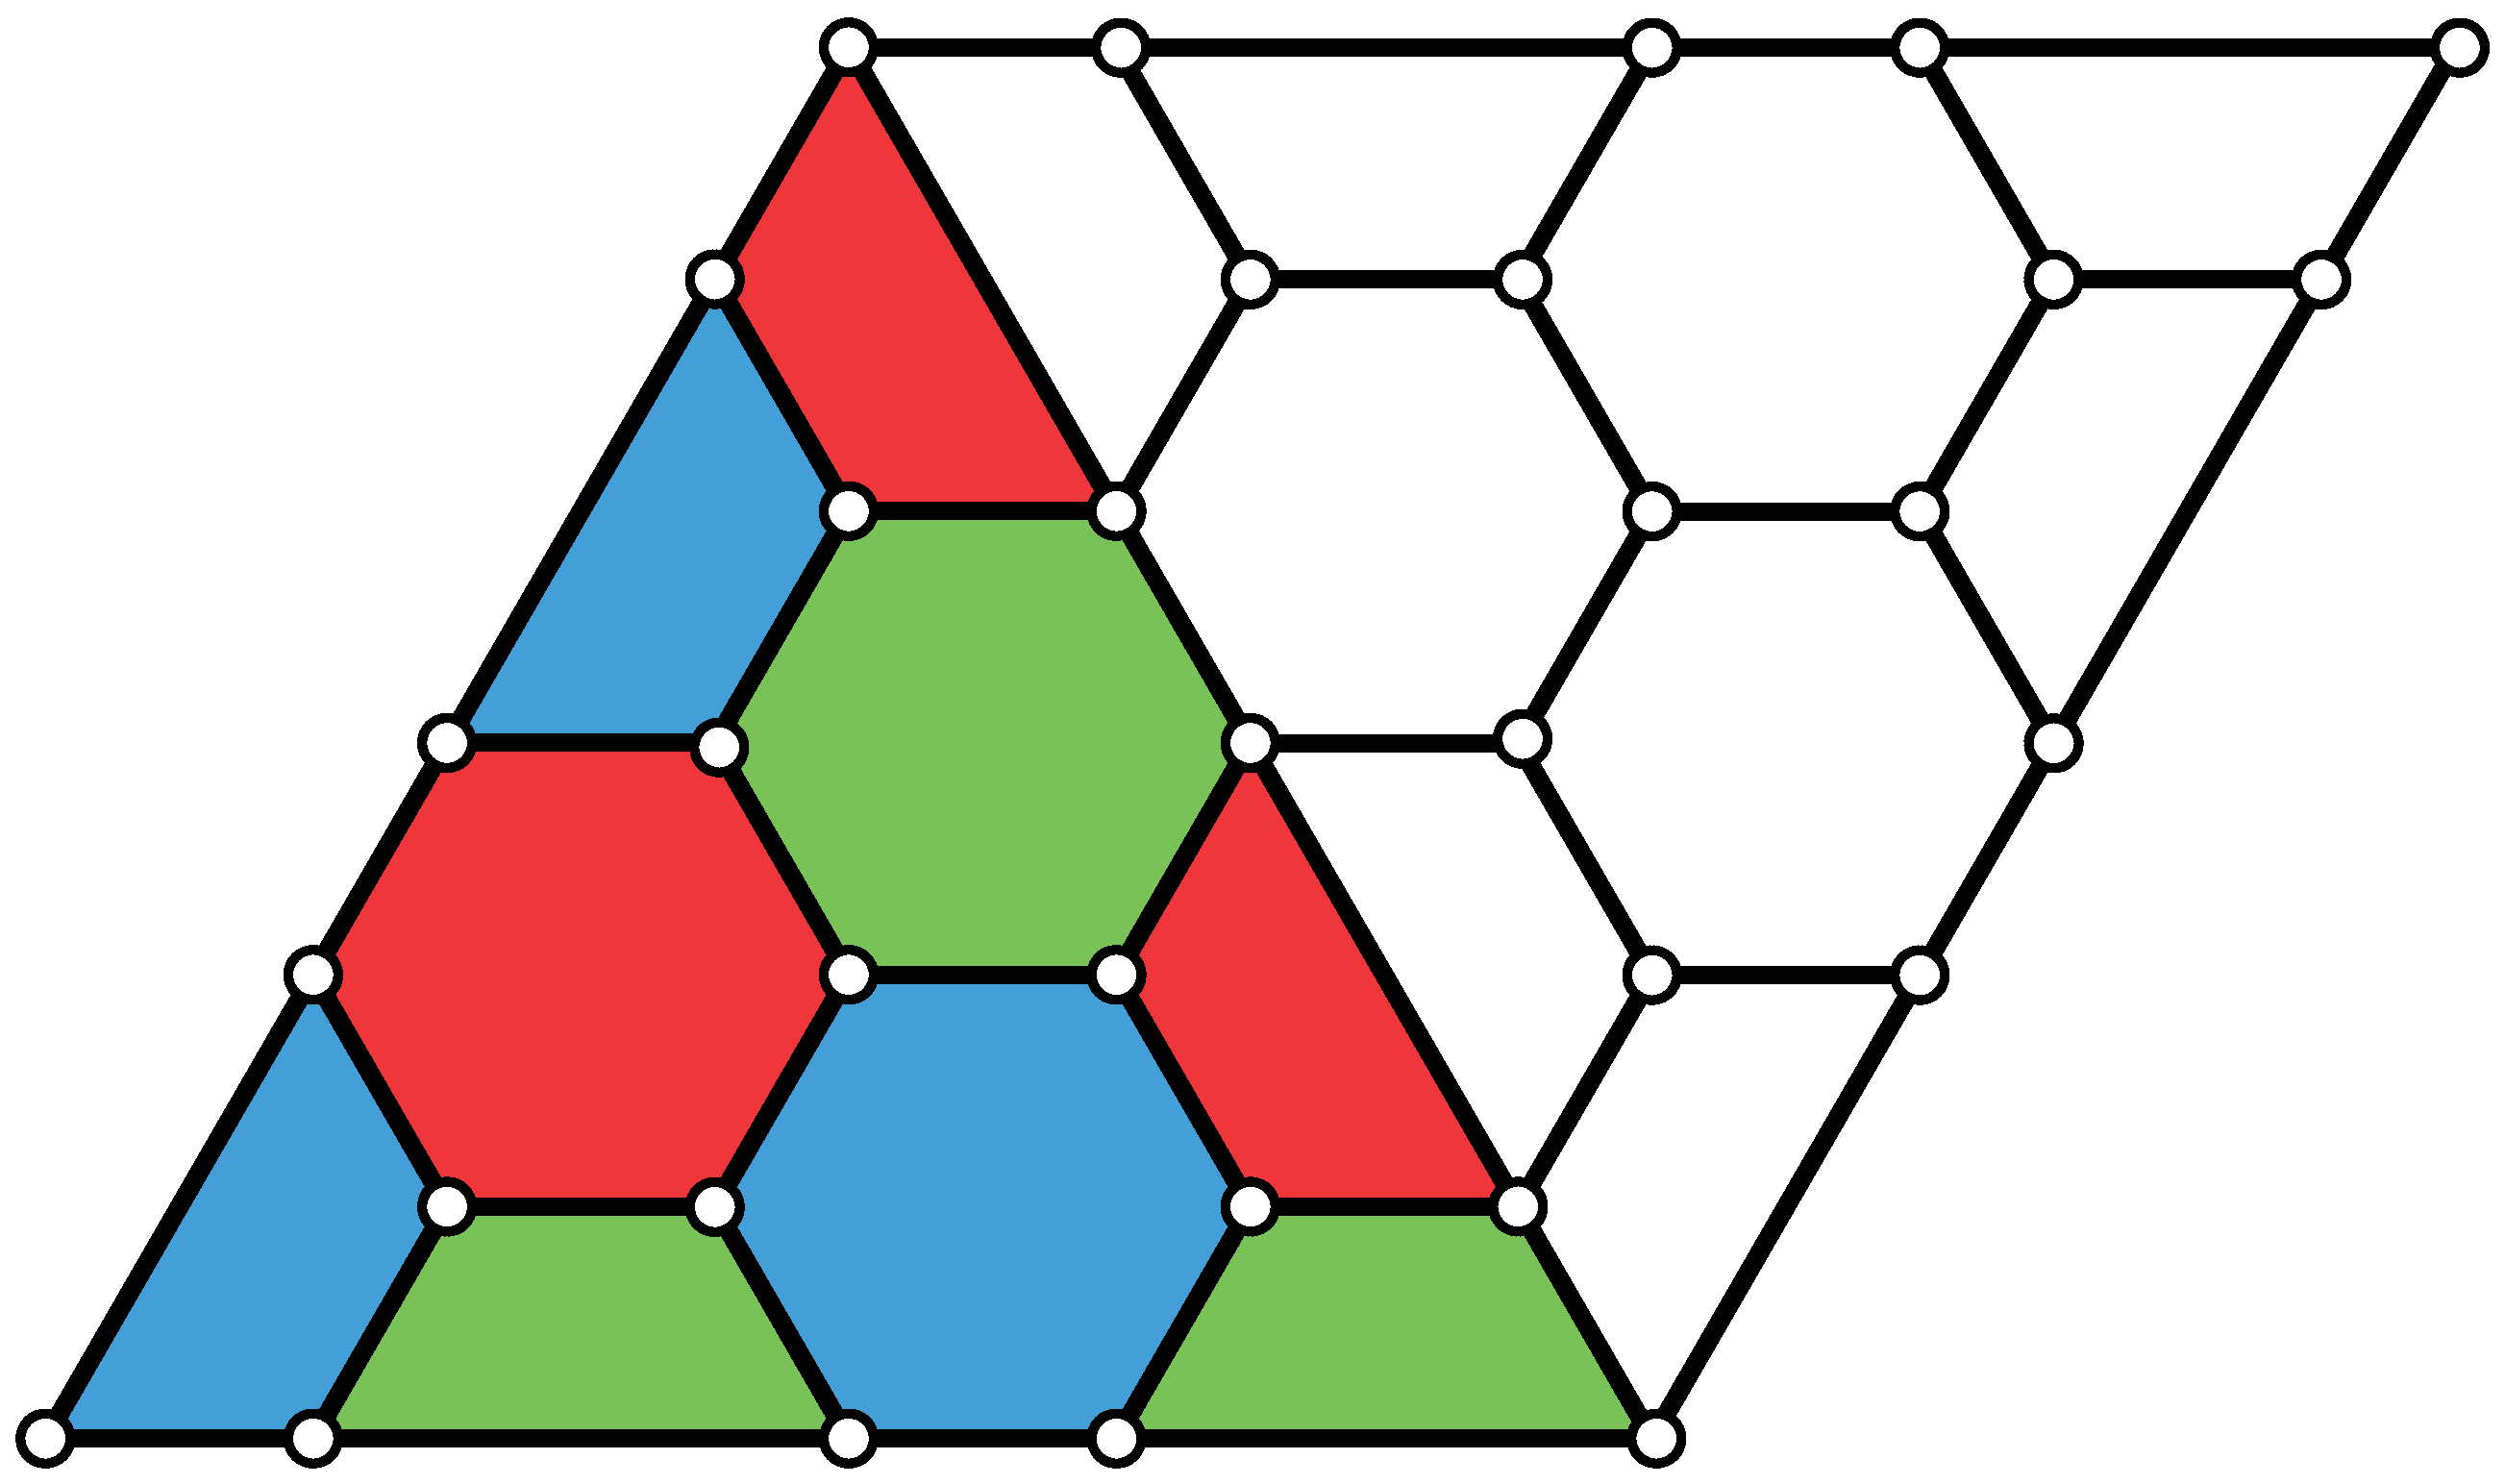
\includegraphics[scale=0.15]{figure/figure2.eps}
        \vspace{10pt}\caption{}
        \label{figure2}
        \vspace{-15pt}
    \end{figure}

    ここでスタビライザー群を$\mathcal{S}$と表す。Fig.\ref{figure3}のようにgreenのedgeにX edge stabilizer、boundary上のblue edgeに対してZ edge stabilizerを$\mathcal{S}$に追加する。ただし、追加された量子ビットの領域に対してもColor Codeが続いているように見て、edge operatorを定義している。これによって、red faceのZ stabilizerは$\mathcal{S}$から消える。またそれと同時に、green faceのX stabilizer、red faceのZ stabilizer、blue faceのZ stabilizerのシンドローム測定を、追加した量子ビットの領域で開始する。そうすると、Fig.\ref{figure3}のようになる。
    \clearpage

    \begin{figure}[h]
        \centering
        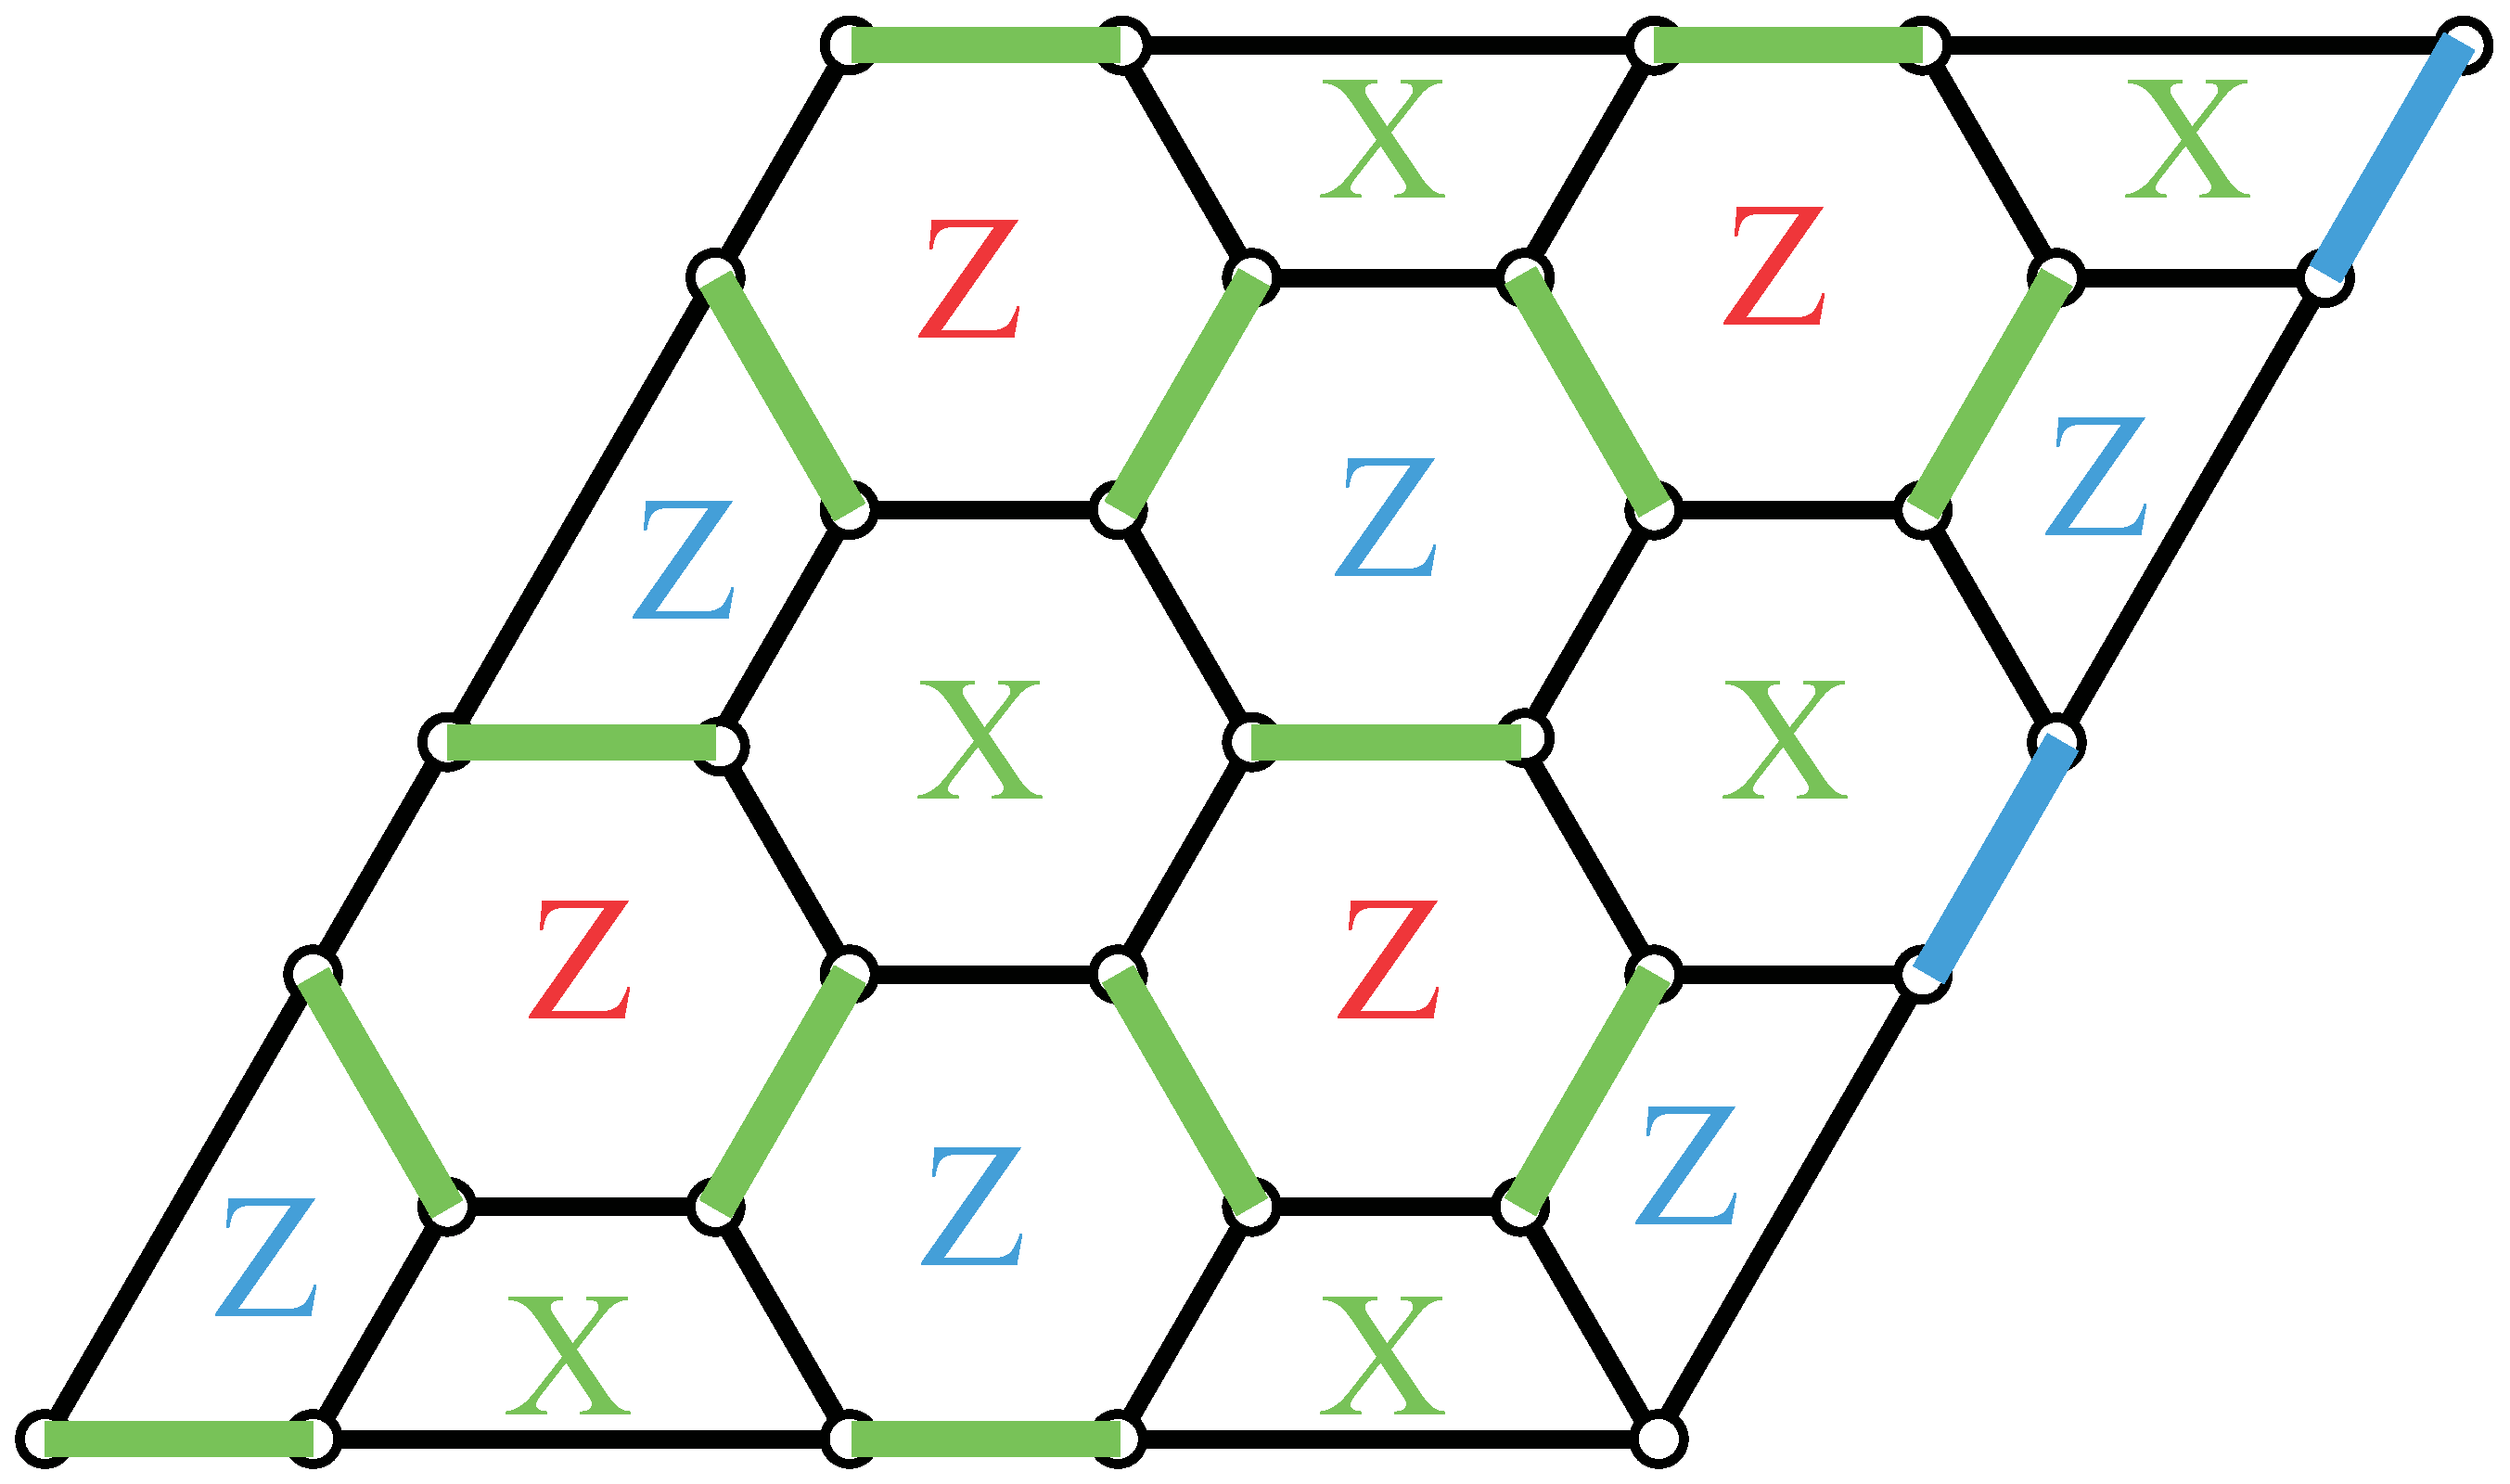
\includegraphics[scale=0.15]{figure/figure3.eps}
        \vspace{10pt}\caption{}
        \label{figure3}
        \vspace{-15pt}
    \end{figure}

    ということで変換後のスタビライザー$\mathcal{S}$はSurface Codeに対応するものとなっており、Fig.\ref{figure4}に示すようになっている。ただし、橙色がX stabilizer、青色がZ stabilizerを表す。ここで定義している6-weightもしくは4-weightのスタビライザーはfloquet code的に実装するのではなく、surface codeのように実際のweight分のシンドローム測定を行う。

    \begin{figure}[h]
        \centering
        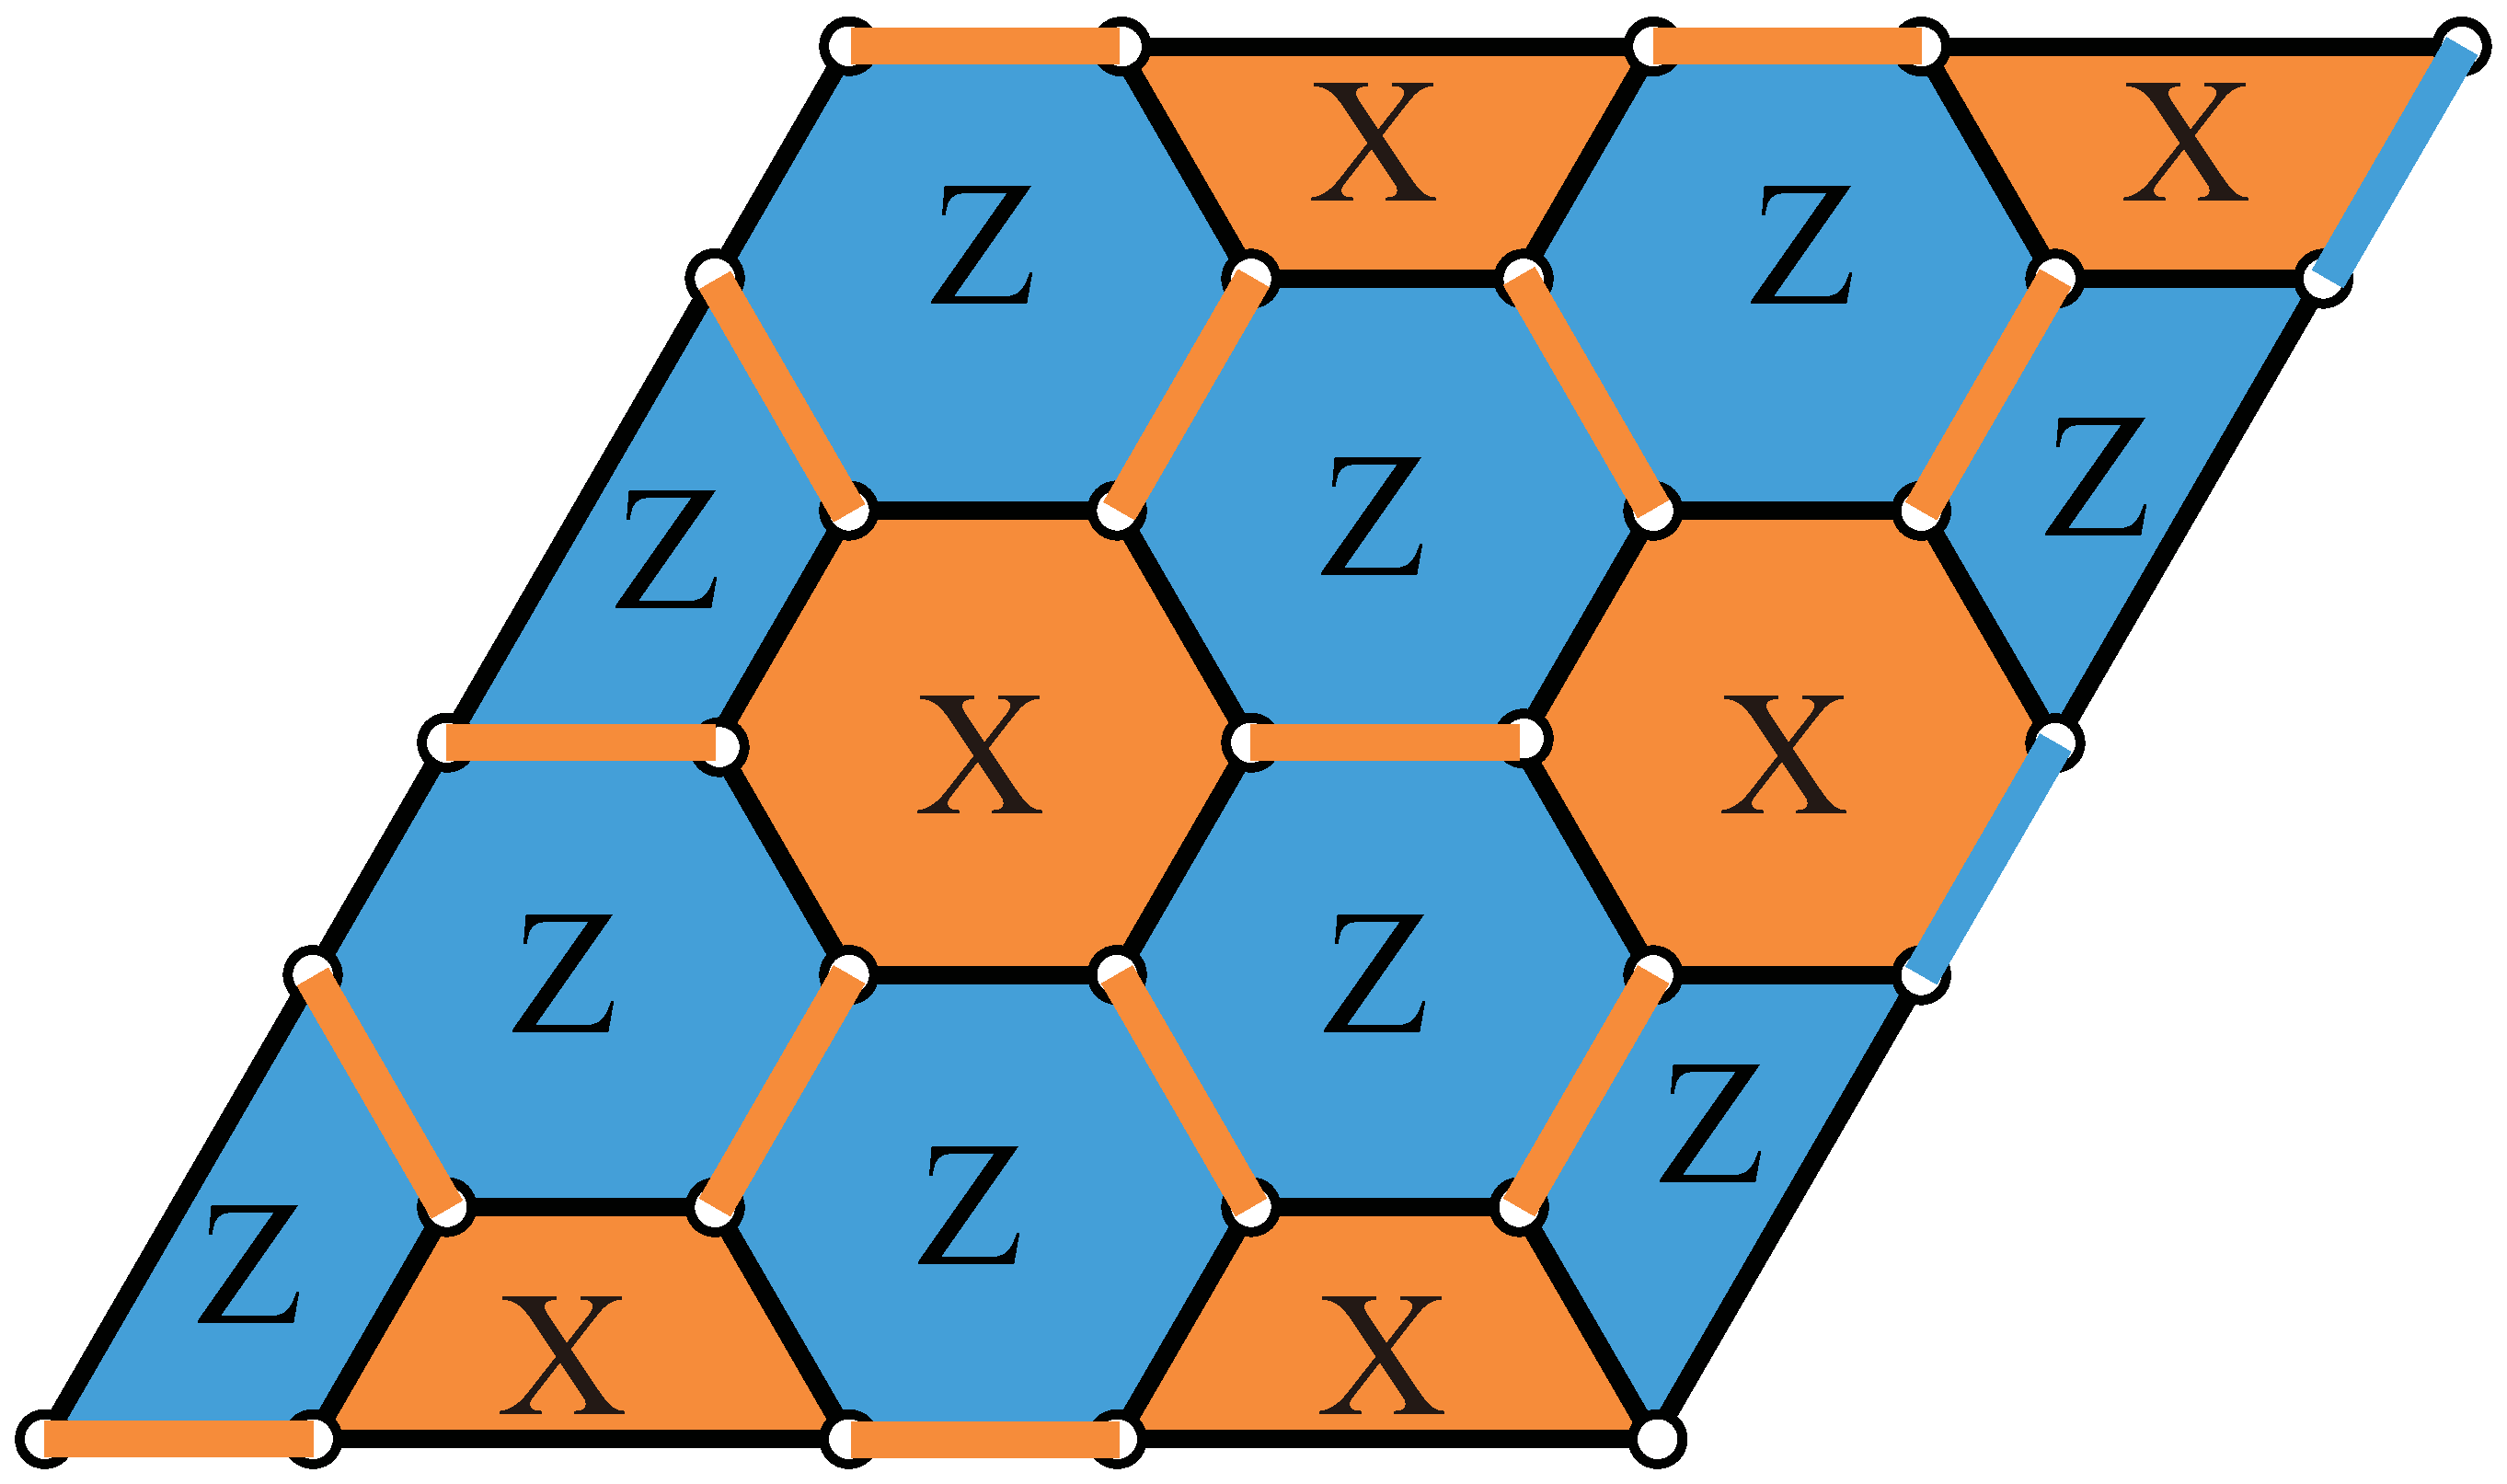
\includegraphics[scale=0.15]{figure/figure4.eps}
        \vspace{10pt}\caption{}
        \label{figure4}
        \vspace{-15pt}
    \end{figure}

    ここで、最初に定義したlogical operatorは追加したすべてのスタビライザーと可換であるため論理情報は保存される(\cite{fu2024}を参照)。
}

\section{拡大}{
     ここまでで、Surface Codeにできたのであとは拡大するだけである。拡大はFowlerとGidneyの\cite{fowler2019}のFig.11と同じようにすればできると思う(Fig.\ref{figure5})。

    \begin{figure}[h]
        \centering
        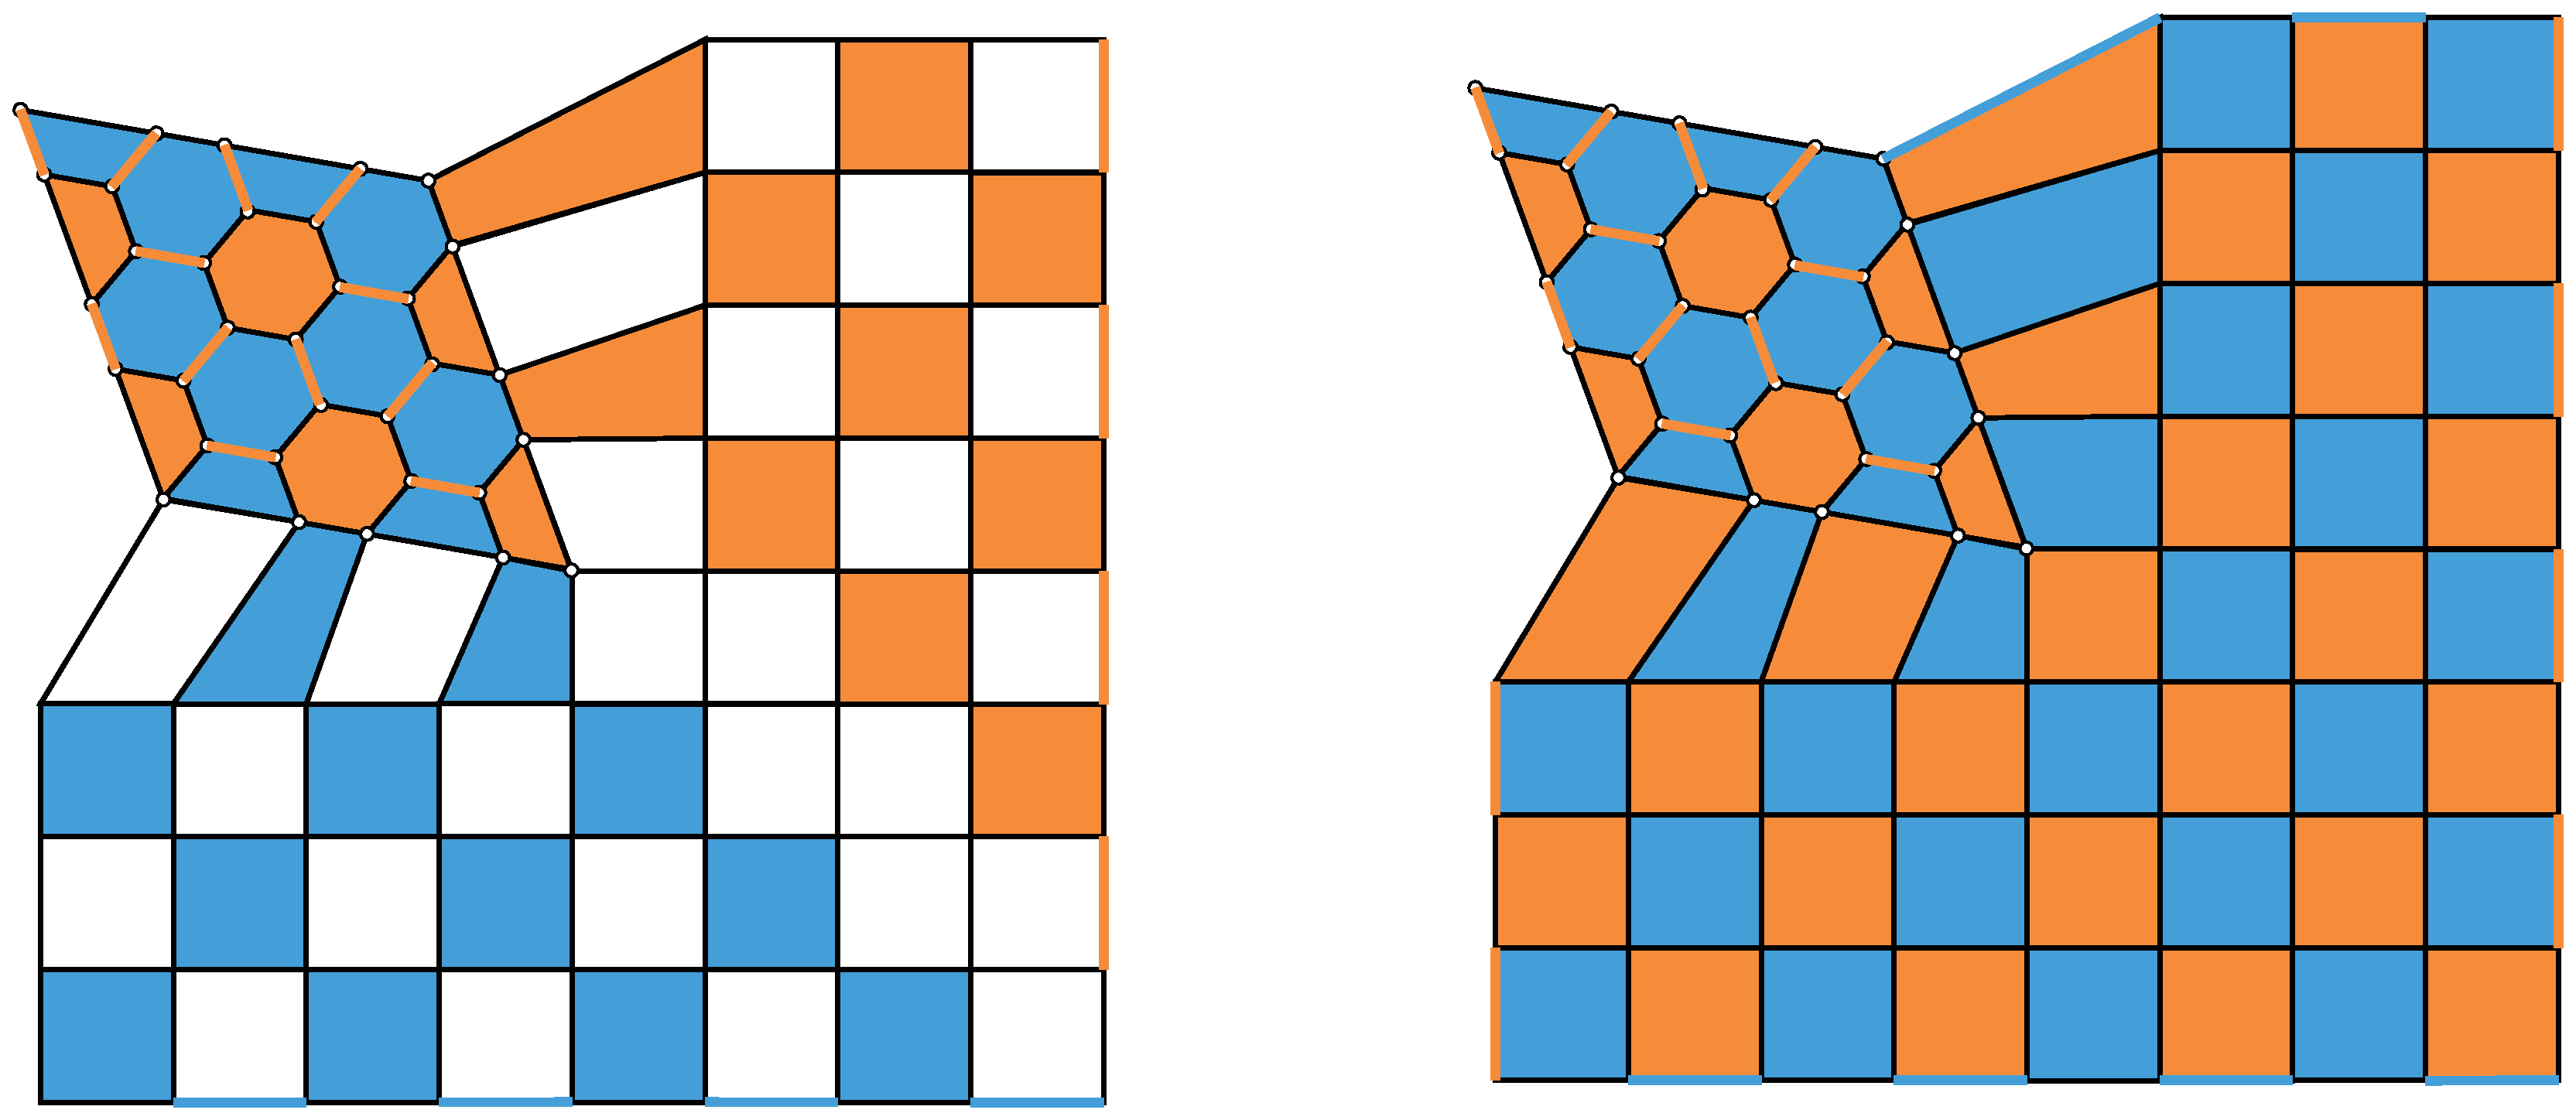
\includegraphics[scale=0.20]{figure/figure5.eps}
        \vspace{10pt}\caption{}
        \label{figure5}
        \vspace{-15pt}
    \end{figure}
    \clearpage
    またここまでの操作はいっぺんにやってしまえば良いので、Fig.\ref{figure6}のように、拡大先のSurface Codeの量子ビットをすべて用意しておいて、その後全体でSurface Codeのシンドローム測定をすることによって、escape stageが完成すると思う。
    \begin{figure}[h]
        \centering
        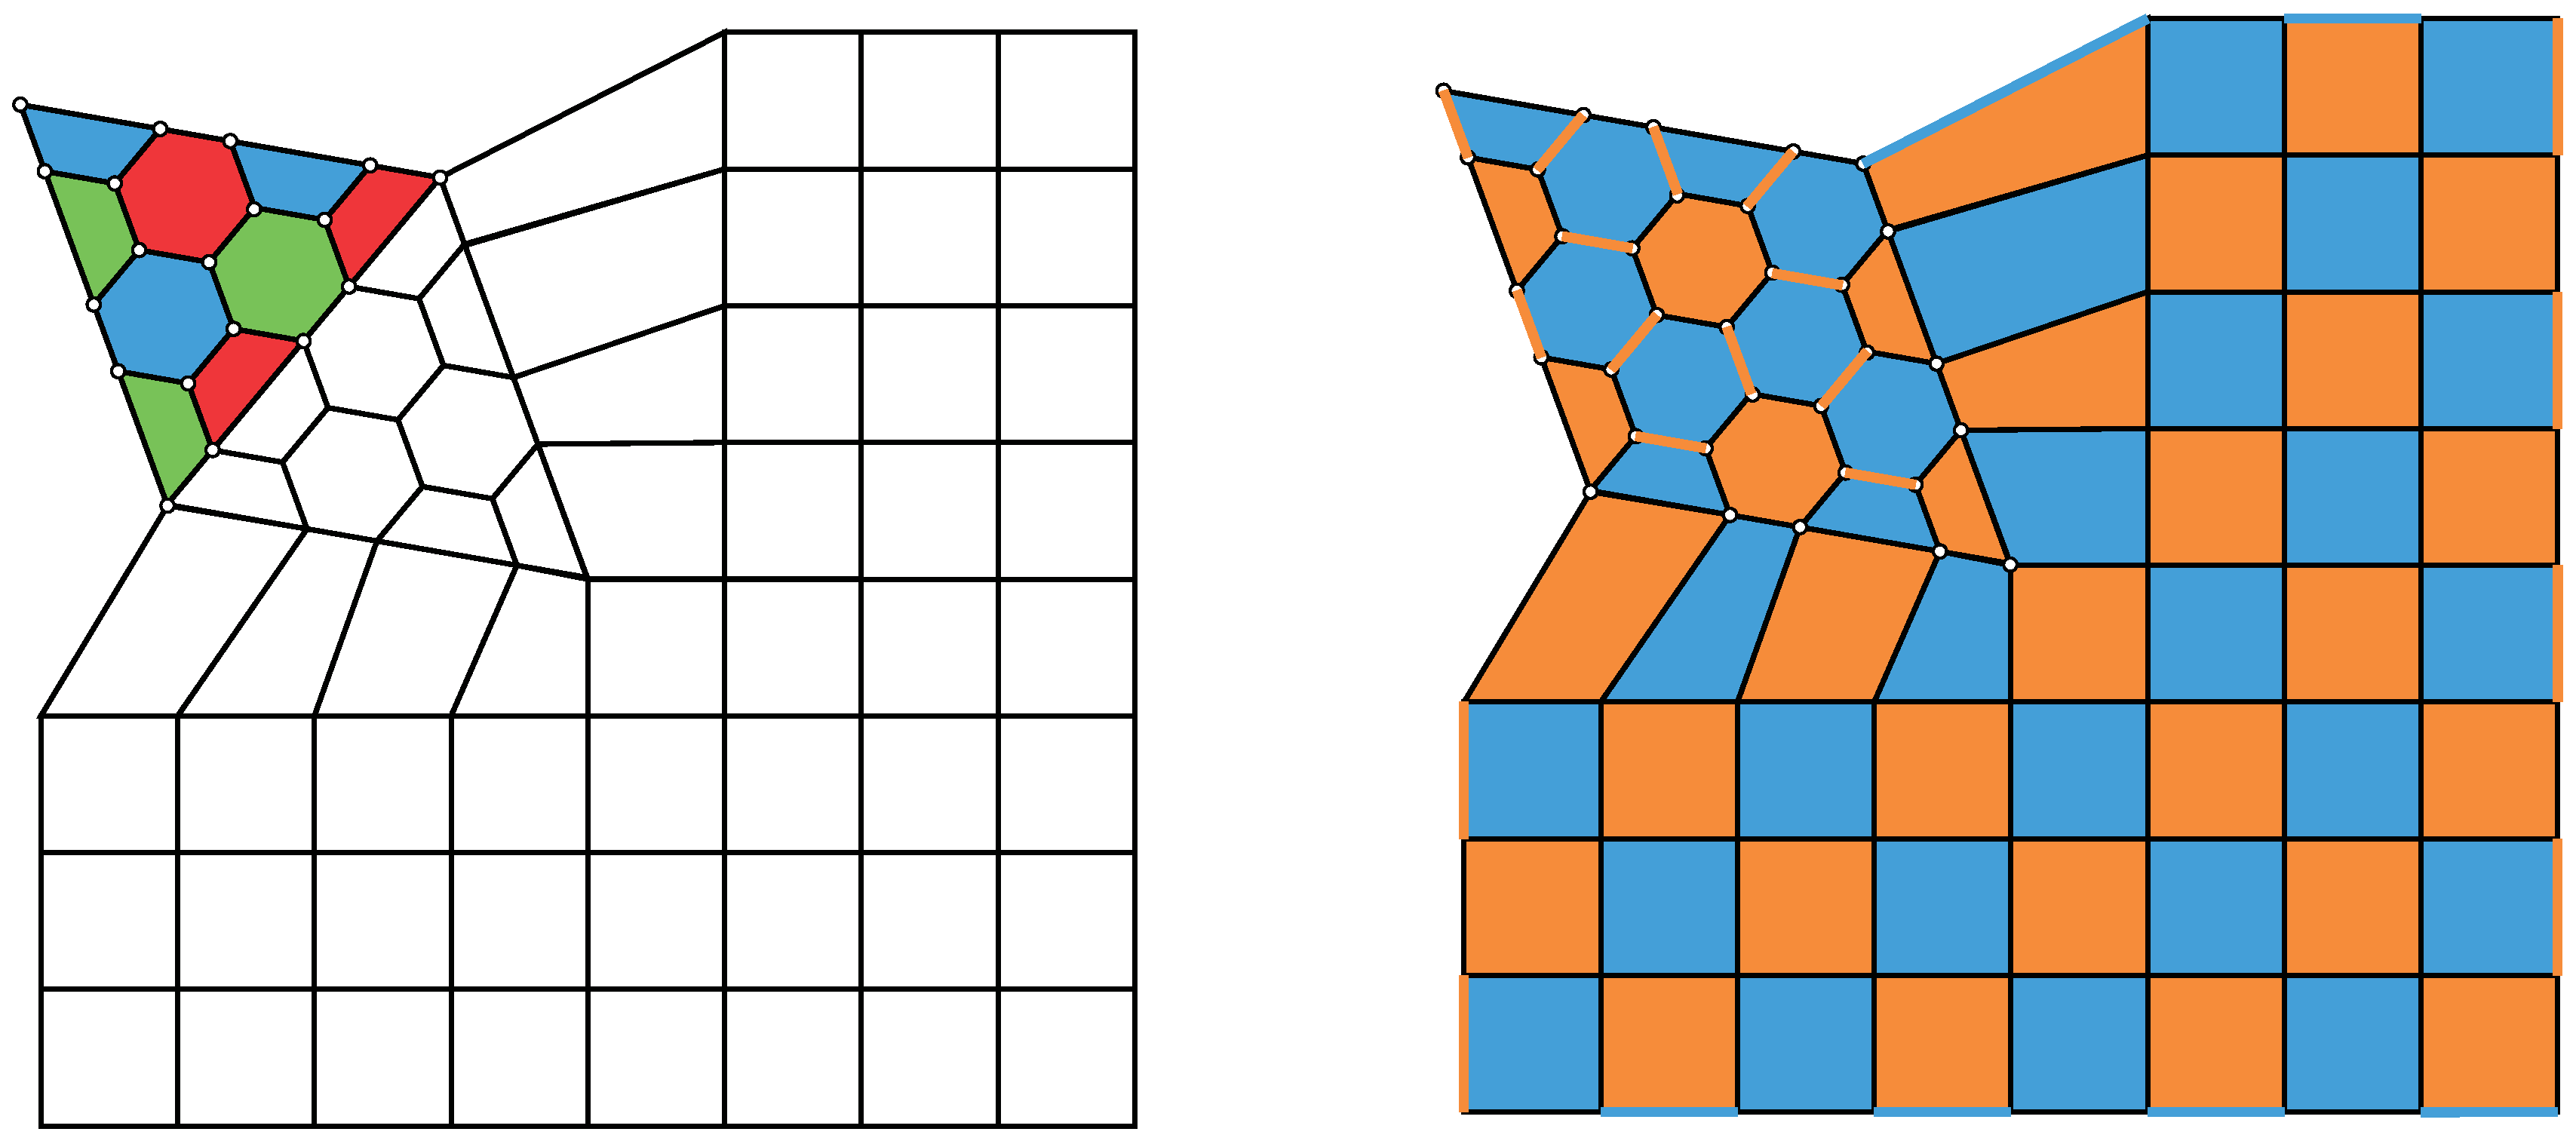
\includegraphics[scale=0.20]{figure/figure6.eps}
        \vspace{10pt}\caption{}
        \label{figure6}
        \vspace{-15pt}
    \end{figure}
}

\section{検証}{
     ここでは、検証を簡単にするために符号距離3の場合について考える。まずはColor CodeからSurface Codeへの変換がエラーが無いときに所望の変換になっているかを検証する。ただし、スタビライザーの測定結果はすべて+が出ることを仮定している。Fig.\ref{figure7}より、Color Codeにエンコードし、Surface Codeに変換する場合と、最初からSurface Codeに変換する場合でLogical OperatorとStabilizerが同じであることがわかる。よって、Color CodeからSurface Codeへの変換は所望の操作になっている。

    \begin{figure}[h]
        \centering
        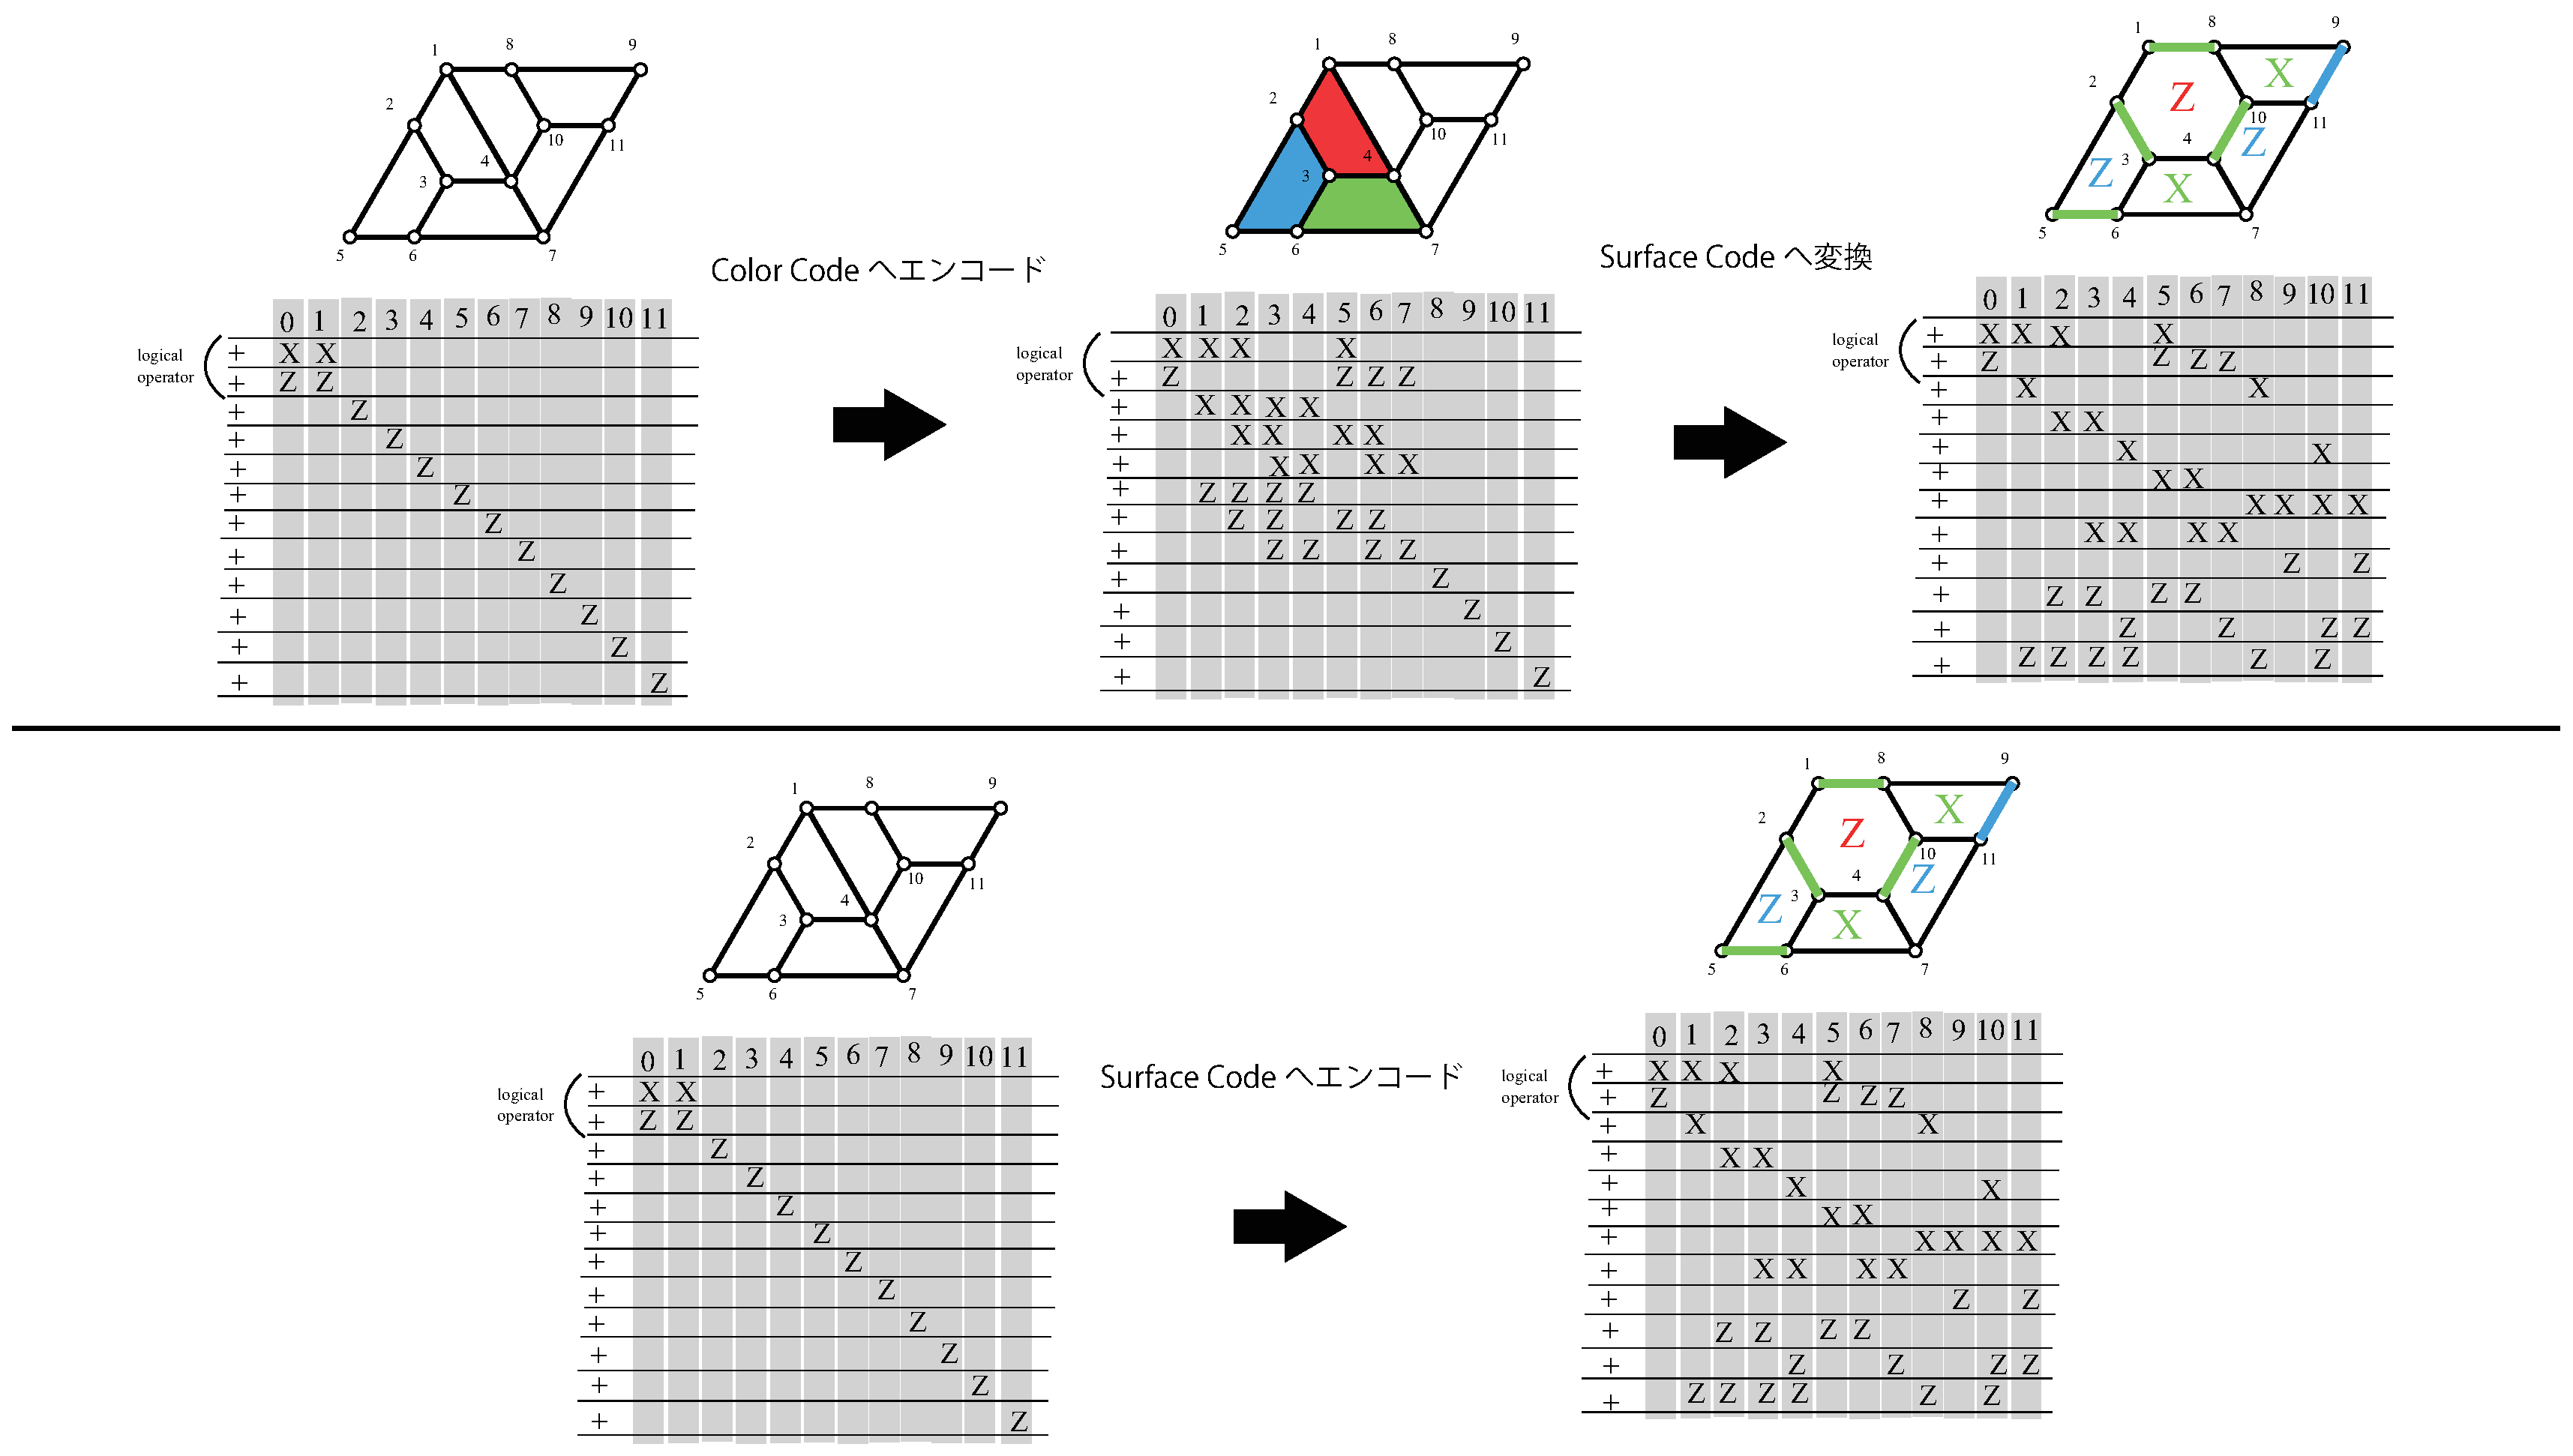
\includegraphics[scale=0.30]{figure/figure7.eps}
        \vspace{10pt}\caption{}
        \label{figure7}
        \vspace{-15pt}
    \end{figure}

    また、拡大操作を検証すると、Fig.\ref{figure8}のようになる。Fig.\ref{figure8}の上段はFig.\ref{figure7}の最終状態から、拡大する操作を表し、下段は拡大されたSurface Codeにエンコードする操作を表す。上段と下段の最終状態は等しいので、拡大操作は所望の操作になっている。

    \begin{figure}[h]
        \centering
        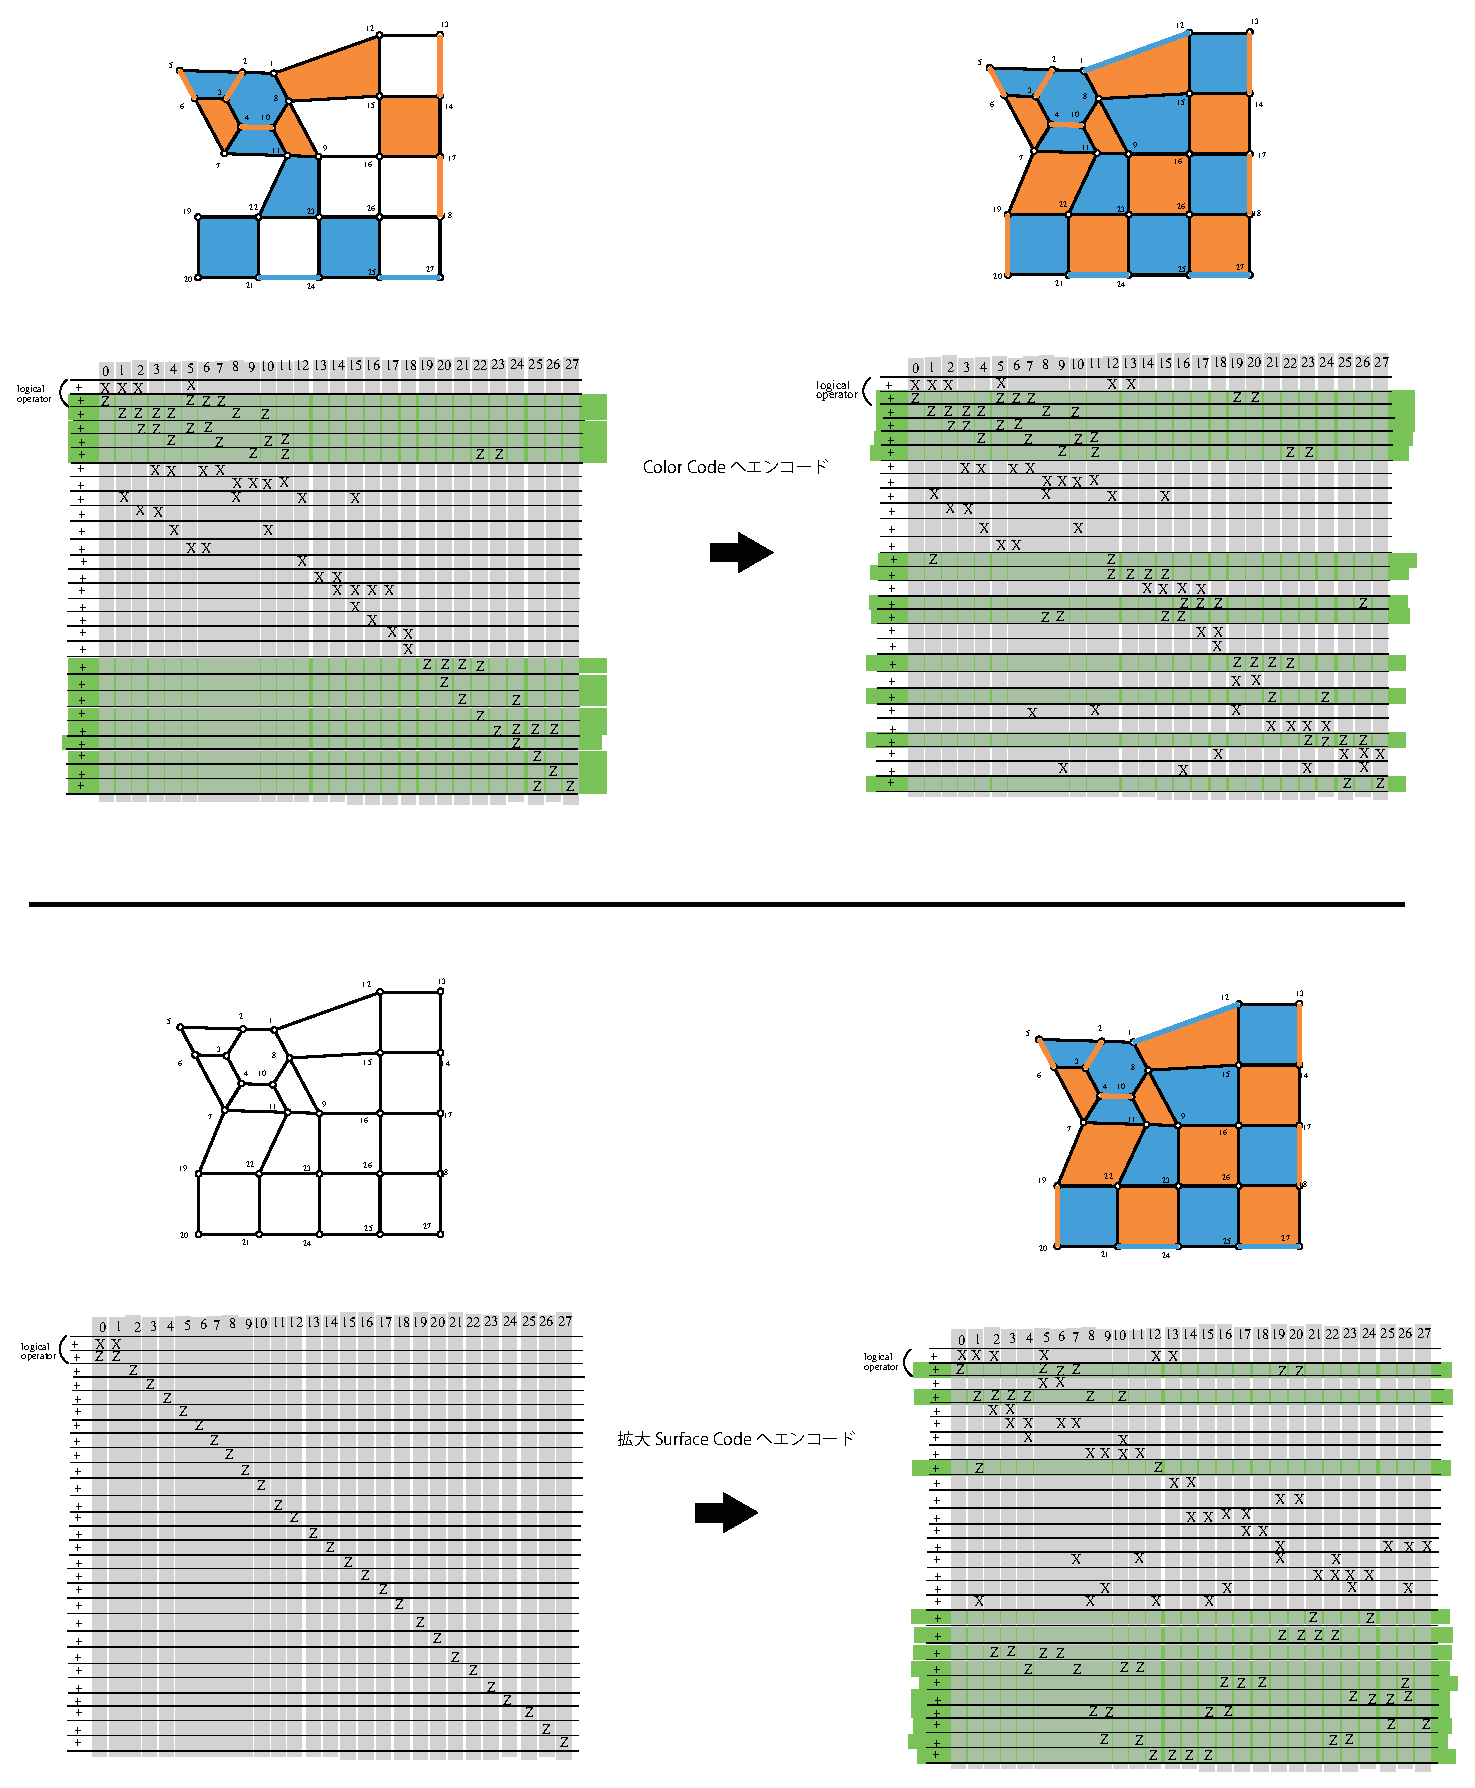
\includegraphics[scale=0.70]{figure/figure8.eps}
        \vspace{10pt}\caption{}
        \label{figure8}
        \vspace{-15pt}
    \end{figure}
    \clearpage

    最後にこれらの操作がいっぺんにできるかを検証する。Fig.\ref{figure9}に示す通り、Color Codeからいっぺんに変換、拡大の操作を行っても、Fig.\ref{figure8}の下段と同じ状態が得られることがわかる。

    \begin{figure}[h]
        \centering
        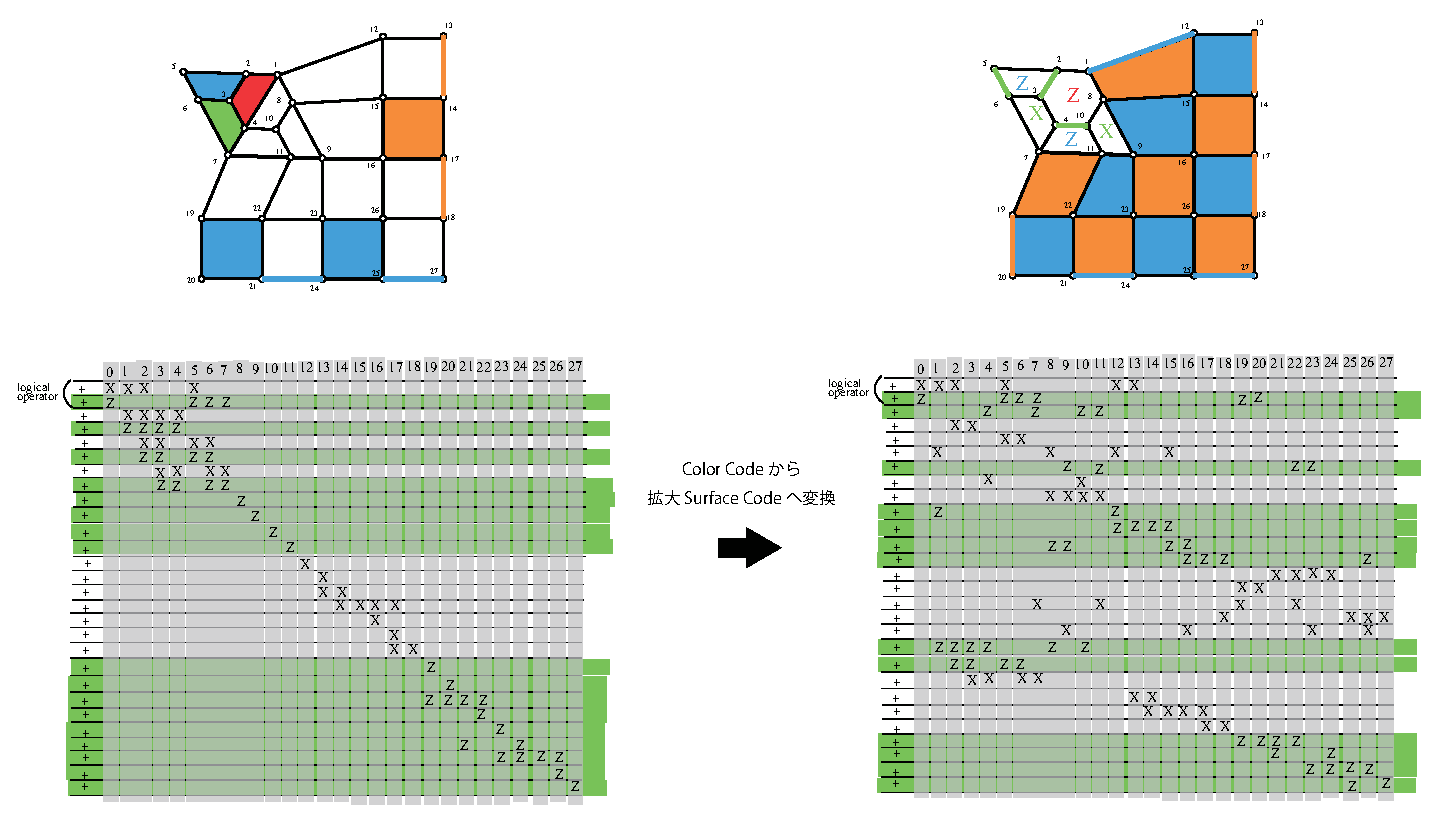
\includegraphics[scale=0.70]{figure/figure9.eps}
        \vspace{10pt}\caption{}
        \label{figure9}
        \vspace{-15pt}
    \end{figure}

}




\printbibliography
\clearpage
Update rules from \cite{fu2024}
\begin{lemma}(\textbf{Stabilizer Update Rules})\label{lemma: stab update rule}

    Let $\mathcal{S}$ be the stabilizer generators with a stabilizer state $\ket{\psi}$ being either in $+1$ or $-1$ eigenstate of the generators. 

Let $m$ be a Pauli measurement performed on $\ket{\psi}$, and denote the outcome of $m$ by $O(m)\in \{\pm 1\}$.

\begin{enumerate}
    \item If $\pm m \in \langle \mathcal{S} \rangle$, then the outcome is fixed by the eigenvalues of stabilizers for $\ket{\psi}$, and the state remains unchanged. 
    \item If $m$ anti-commutes with some elements in $\mathcal{S}$: Let $V = \{s_1, s_2,\cdots, s_l\}$ be a subset of $\mathcal{S}$ whose elements anti-commute with $m$. We replace $s_1$ with $m$ and update the rest of $V$ by $s_i \to s_i \cdot s_1$, for $2 \leq i\leq l$. $\mathcal{S} \cap V$ is now updated to $ \{O(m) \cdot m, s_2\cdot s_1, s_3 \cdot s_1,\cdots, s_l\cdot s_1\}$ 
    \item If $\pm m \notin \langle \mathcal{S} \rangle$ and $[m,s]=0 \, \forall s \in \mathcal{S}$, then we update the set of stabilizer generators: $\mathcal{S} \to \mathcal{S} \cup \{O(m) \cdot m\}$. This assumes that $m$ is not a logical operator. 
\end{enumerate}
\end{lemma}

\begin{lemma}(\textbf{Logical Update Rules})\label{lemma: logical update rule}

Let $L$ be a logical operator of a stabilizer group $\langle S\rangle $ and let $\ket{\psi}$ be an eigenstate of $L$.

Let $m$ be a Pauli measurement performed on $\ket{\psi}$ and denote the outcome by $O(m) \in \{\pm 1\}$.
\begin{enumerate}
    \item If $m = (-1)^a \cdot L$, then $O(m)\cdot (-1)^a$ gives the eigenvalue of $L$ for the state $\ket{\psi}$, and the logical operator remains unchanged. 
    \item If $m$ commutes with $L$, the logical operator remains unchanged. 
    \item If $m$ anti-commutes with $L$ and commutes with $\langle S\rangle $, then $L$ is updated to $O(m) \cdot m$. The new state is a $+1$ eigenstate of $O(m) \cdot m$ instead of $L$.
    \item If $m$ anti-commutes with $L$ and anti-commutes with some elements in $S$: In the stabilizer update rules, we replace an element $s_1$ with $m$ and update the rest of the elements in $S$ that anti-commute with $m$ using the $ 2^{\mathrm{nd}} $ rule in Lemma \ref{lemma: stab update rule}. For the logical operator, we update $L\to L\cdot s_1$, where $s_1$ is the element that is replaced with $m$.
\end{enumerate}
\end{lemma}
\end{document}